\documentclass[../main.tex]{subfiles}
\begin{document}
\section{Corrections to simulated events}
\label{hh:sec:corrections}

\subsubsection*{Pile-up reweighting}
\label{hh:sec:pu}

The production of additional objects coming from PU vertices can lead to significant variations in the analysis results. Therefore, the effect of additional proton-proton interactions is also modelled in simulated events by including final state particles produced in minimum bias events. The probability distribution of the number of PU interactions is modelled before the data taking period itself, so it may not reflect the exact PU distribution of the data. Then, simulated events have to be weighted according to the ratio between the PU distributions of data and MC. \textcolor{red}{Shall I include the distributions? Probably I have to plot them myself.}


%\begin{figure}[h!]
%\begin{center}
%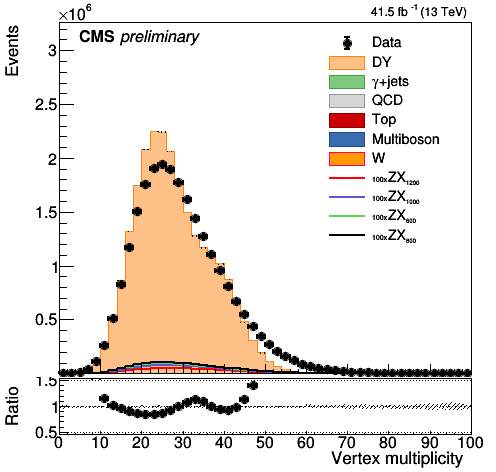
\includegraphics[width=0.5\textwidth]{Images/nvtx_mm.png}
%\end{center}
%\caption{Distribution of number of PU vertices in 2017 for both data and simulated samples.}
%\label{hh:fig:pu}
%\end{figure}

\subsubsection*{Pile-up jet identification scale factors}

As described in Section~\ref{hh:subs:jets}, jets with $p_t < 50$~GeV only are considered if they pass the loose working point of the pile-up jet ID discriminator. As this discriminator is not 100\%(0\%) efficient on real(PU) jets and its results can differ between data and MC events, some scale factors are needed to weight the MC events. These scale factors are produced by studying the efficiency, i.e. probability of a real jet (a reconstructed jet matched to a MC generator-level jet) to pass the PU jet ID working point, and the mistag rate, i.e. the probability of a PU jet (a reconstructed jet not matched to a MC generator-level jet) to pass the PU jet ID working point.

\subsubsection*{Jet smearing}

Measurements have shown that the jet energy resolution (JER) in data is worse than in simulation \cite{hh:cor:smearing_8TeV}. Then, jets in simulated events need to be smeared to describe the data. The smearing procedure consists on a hybrid method used to scale the reconstructed four-momentum of a jet with an scaling factor $f$. First, a matching is performed between the jet and a generator-level jet if $\Delta R(\text{jet}, \text{genjet})<0.2$ and $|p_T^{\text{jet}} - p_T^{\text{genjet}}| < 3\sigma p_T^{\text{jet}}$, where $\sigma$ is the relative jet momentum resolution measured in data. In case this matching is performed, the scaling factor $f$ is obtained as
\begin{equation}
f = 1 + (s - 1)\frac{p_T^\text{jet} - p_T^\text{genjet}}{p_T^\text{jet}},
\end{equation}
where $s$ is the data-to-simulation core resolution scale factor. Otherwise, $f$ is obtained in an stochastic approach as
\begin{equation}
f = 1 + N(0, \sigma)\sqrt{\max(s^2-1, 0)},
\end{equation}
where $N(0, \sigma)$ is a random number sampled from a normal distribution with zero mean and $\sigma$ standard deviation.

\subsubsection*{Level-1 ECAL prefiring}

In 2016 and 2017 operation, a slowly developing shift in the shape of the ECAL pulses was observed \cite{intro:l1_13tev}. This effect was manifested in an increasing offset in the timing calibration of the pulses, affecting mostly the endcap crystals. This effect was compensated offline by recalibrating the pulses, but was not corrected in the ECAL TPs. With time, this effect ended up moving the endcap pulses to a time region where the bunch crossing assignment would be affected, leading to the Level-1 trigger system to \textit{prefire}, i.e. accept the earlier collision in BX - 1, whereas the one in BX 0 is the one of interest. Since Level-1 trigger rules forbid two consecutive bunch crossings to fire, the actual event could be skipped. This effect was not account for by the simulations, so additional weights are included to account for the probability of an event to prefire according to the $p_T$ and $\eta$ of forward jets and photons in the event.

\subsubsection*{Trigger efficiency scale factors}
\label{hh:sec:trigger_sf}

The efficiencies obtained in the single-lepton, cross-lepton and VBF trigger used in the analysis yield to discrepancies between data and simulation, which can be compensated by including some event weights, so-called trigger scale factors. For the \tauh\tauh{} final state, trigger efficiencies and scale factors are measured using Z$\to$\taumu\tauh{} events selected with a tag and probe technique. For the semi-leptonic final states, the SFs must take into account the logical OR of the single-lepton and cross-lepton triggers. Assuming the lepton and \tauh{} legs are independent, the efficiency for both simulation and data can be obtained as
\begin{equation}
\text{Eff} = \epsilon_L(1-\epsilon_{\tau_h}) +  \epsilon_l\epsilon_{\tau_h},
\end{equation}
where $\epsilon_L$ is the single lepton trigger efficiency, $\epsilon_l$ is the cross lepton trigger efficiency for the \taue{} or \taumu{} leg and $epsilon_{\tau_h}$ is the cross lepton trigger efficiency for the \tauh{} leg.

For the VBF trigger paths, efficiencies and scale factors are computed separately for the \tauh{} legs and the jet legs. For the first ones, they are applied as a function of the $p_T$ and decay mode of the two \tauh{}, while for the latter, on the transverse momenta of the two jets with the highest invariant mass and on the actual invariant mass. Note that these VBF trigger scale factors are only applied in the VBF phase space, i.e. where one of the \tauh{} has a $p_T$ between 25 and 40~GeV. If both \tauh{} have a $p_t>40$~GeV, the $\tau_h\tau_h$ scale factors are considered instead.



\subsubsection*{Trigger prescale weights}
\label{hh:sec:prescale_sf}

In order to account for the trigger prescales used for data taking for some of the HLT paths, the simulated events that fired only prescaled paths are corrected with weights obtained as the ratio between the integrated luminosity covered by the prescaled trigger over the total integrated luminosity of the year. 

\subsubsection*{b-tagging efficiency}

To account for discrepancies in the b-tagging performance of the DeepJet algorithm between data and simulation, the discriminant distribution is corrected by applying weights to the simulated events. These weights are obtained as
\begin{equation}
w = \prod_i^{N} SF(D^i, p_T^i, \eta^i),
\end{equation}
where the product considers all jets satisfying the requirements described in Section~\ref{hh:subs:jets}. The scale factors are produced as function of the discriminator score, the $p_t$ and the $\eta$ of the jet.

As stated before, these additional weights intend to only modify the shape of distribution, not the expected event yields. As only applying these weights could lead to modification on the total event yields, the final distributions are corrected by scaling with the ratio of the sum of event weights without considering the b-tag weight and considering it.

\subsubsection*{\deeptau{} scale factors}

The \deeptau{} algorithm shows small differences when running it on data or simulated events. To account for these differences, some scale factors are included depending on if a genuine $\tau_h$ or a misidentified particle is selected as the $\tau_h$. For genuine $\tau_h$, scale factors are provided binned in the \tauh{} $p_t$. For genuine electrons misidentified as $\tau_h$, scale factors are provided split into barrel and endcap, while for genuine muons, binned as a function of $\eta$.

\subsubsection*{Electron and muon scale factors}

To account for possible disagreements between data and simulation regarding the reconstruction and identification of muons and electrons in the \taumu\tauh{} and \taue\tauh{} channels, specific scale factors binned in the lepton $p_t$ and $\eta$ are provided.

\subsubsection*{Tau Energy Scale}

The correction to the $\tau_h$ energy scale is defined by the deviation of the average reconstructed $\tau_h$ energy from the generator-level energy of the visible \tauh{} decay products \cite{tau_performance_2018, tau_performance_2022}. The data-to-simulation correction factor is obtained by fitting distributions of observables sensitive to the energy scale in Z/$\gamma^*\to\tau\tau\to$~e\tauh,$\mu$\tauh{}, such as the $m_{\tau_h}$ and the mass of the $l\tau_h$ system. These corrections modify the energy and momentum on the $\tau_h$, modifying also the shape of the final discriminants. Four independent corrections are provided, one for each decay mode used in the analysis, taking values of up to 2\%. 

~\\

\textcolor{red}{Shall I mention the 2017 custom scale factors? Not mentioned in the paper but in the AN}


\end{document}

